% Chapter 1
\begin{savequote}[10pc]
\sffamily 
``The issue is no longer where the information lives - what server, what
application, what database, what data center. It's actually now all about putting
information to work.''
\qauthor{Carly Fiorina (1954-)}
\end{savequote}
\chapter{Google App Engine}\label{chap:gae}
When creating Web applications there is an overhead going from development into
production with the application. The overhead includes setting up several
elements: a Web server, a database, scripts, monitoring, etc. In this chapter, we
introduce and describe the Google App Engine (GAE) which removes the
overhead. We describe the GAE architecture, and based on the description we
present snippets of Web application code and assemble them into a working GAE
application.

\section{What is the Google App Engine?}
GAE is a server and development platform, created by Google. GAE lets programmers
focus on crafting the application and eliminates many server issues. GAE reduces
the time to deploy and automatically scales as the application grows by
providing access to the Google infrastructure. The infrastructure consists of a
serving infrastructure and several Google services, such as
\textit{\gls{gls:googleaccounts}} and the datastore.

The serving infrastructure is encapsulated away from the application
programmer. Behind the scenes, the infrastructure adjusts the resources allocated
to serve the application, depending on the load on it. Outsourcing the serving
infrastructure to Google has the advantage that issues about serving the
application are moved to experts at Google. Server issues include things such as
setting up the server, securing it, making it scale, etc.

Before the programmer can focus entirely on creating the application, there are
still issues regarding both bringing the application online and debugging the
application. Google has put an effort into solving these issues by creating a
local development environment and scripts to bring the application online
instantly.

The advantages come at a cost; a GAE application is limited in numerous ways
\citep{Google:quota, Google:cgi}. In February 2009, the limitations were quite
severe:
\begin{itemize}
  \item only one language was supported, namely Python;
  \item scheduling tasks were impossible, since HTTP requests were the only means
  to start a process; and
  \item long-lasting processing was impossible, since requests could not last longer
  than 10 seconds.
\end{itemize}
Google App Engine is an emerging technology; since the first writing, five months
ago, the GAE is changed in numerous
ways: Google has since added Java support\footnote{\url{http://code.google.com/p/googleappengine/issues/detail?id=1}
}, scheduling of cron jobs\footnote{\url{http://groups.google.com/group/google-appengine/browse_thread/thread/552e9ab4a97abc48?hl=en}
}, however, limited to 20, and increased
the request duration to 30 seconds\footnote{\url{http://code.google.com/p/googleappengine/issues/detail?id=6}
}, and etc..

The limitations are now mitigated, however, essential tasks still \textit{cannot}
be done. The limitations mean that many GAE applications demand workarounds;
thus, when to use GAE is a subjective matter that depends on the type of the
application.

On the other hand, GAE is free and makes it easy to get started with one's
application. Therefore, for a prototype Web application that fit almost within
the limits of GAE, the advantages outweigh the disadvantages, and make GAE
suitable.


%A benefit of GAE, unlike other similar offerings, such as Amazon Elastic Compute
%Cloud\footnote{\url{http://aws.amazon.com/ec2/}} and Aptana
%Cloud\footnote{\url{http://www.aptana.com/cloud}}, is that it is free.
%% Aptana Cloud has no cron job either!!! http://forums.aptana.com/viewtopic.php?f=43&t=5935

\section{An example for the impatient}
Before digging into the GAE architecture we show a 'Hello, world' example for
GAE. The interesting point about the example is how little code is needed to run
the example on the server.

The 'Hello, world' example consists of only two files, given in
Listing~\ref{lst:appYamlHelloWorld} and Listing~\ref{lst:helloWorld}.

\begin{itemize}
  \item \verb|app.yaml|, a configuration file containing handlers. Handlers are a
  list of \textit{\gls{gls:uri}} patterns with descriptions of how requests to \gls{gls:uri}s are handled. In
  this case the server will execute the script \verb|main.py| for all \gls{gls:uri}s. %
  \item \verb|main.py|, a Python \textit{\gls{gls:cgi}} script that output a
string containing a content header and the content, which the server sends back
to the client.
\end{itemize}

\begin{lstlisting}[caption=app.yaml,label=lst:appYamlHelloWorld]
application: helloworld
version: 1
runtime: python
api_version: 1

handlers:
- url: .*
  script: main.py
\end{lstlisting}


\begin{lstlisting}[caption=main.py,label=lst:helloWorld]
print 'Content-Type: text/html'
print                            # end of headers
print '''
<html>
  <head>
    <title>Hello, world</title>
  </head>
  <body>
    <h1>Hello, world</h1>
  </body>
</html>
'''
\end{lstlisting}

The example is run by starting the development server, with the directory of the
two files, as argument. Now accessing \verb|http://localhost:8080| with a
browser outputs \verb|Hello, world|.

\section{Architecture}
\begin{figure}[htbp]
  \centering
  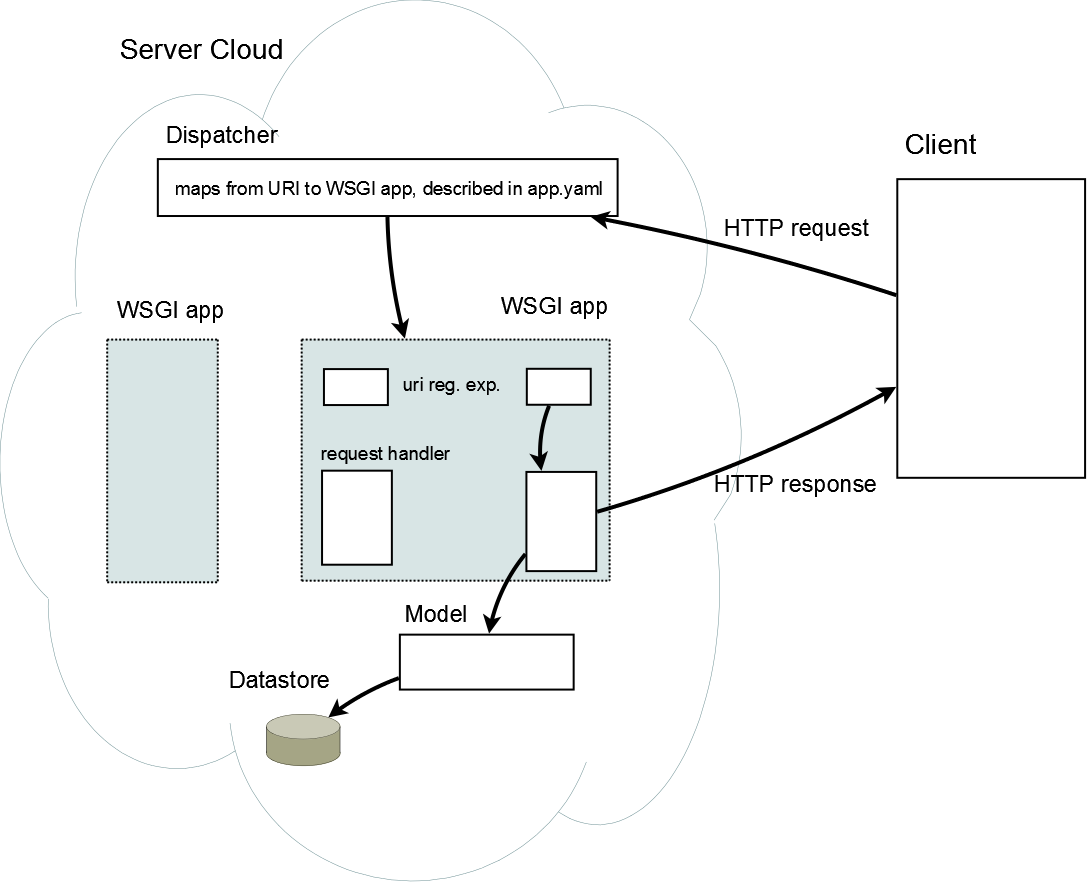
\includegraphics[width=\textwidth]{./Figures/webappArch}
%  \rule{\textwidth}{0.005in}
  \caption{GAE architecture}
  \label{fig:webapp}
\end{figure}
%%The GAE roughly consisting of five things:

%%\begin{enumerate}
%%  \item a serving infrastructure, which connects \gls{gls:uri} requests to a running
%%  instance of the application code somewhere in the %%
%%
%%   \xglossary{name={server cloud}, 
%%              description={ToDo}}%
%%             {\textit{server cloud;}} 
%% %%
%%   \item a Python runtime environment;
%%   \item an SDK which supports development and running of the code locally;
%%   \item administration tools; and
%%   \item the Google database, called datastore.
%% \end{enumerate}

The basic architecture of GAE is illustrated in Figure~\ref{fig:webapp}. Starting
from the client, on the right, incoming \gls{gls:uri} requests are routed to a
corresponding \textit{\gls{gls:wsgi}} application -- the blue squares in the
figure -- somewhere in the server \textit{\gls{gls:cloud}}. Inside the WSGI
applications the requests are routed again to a request handler, which
potentially interacts with the data models, to get relevant data. At last the
server returns a string to the client.

The GAE comes with its own Web application framework called webapp. The Web
server supports any \textit{CGI}-compliant Python application, like webapp or
Django. However, since Django is tied closely together with relational databases,
the Django framework cannot directly be used in GAE. There are different helpers
to work around the database impedance mismatch
\citep{Google:djangohelper,GAE:djangopatch}. For the application in this thesis
we are using the app-engine-patch that adds Django support to GAE.

Crafting Web pages in Django follows the
\textit{\gls{gls:requestresponsepattern}} from HTTP. A Django application
contains request handlers which are Python functions. When a request arrives in
the Django application, it is routed to a request handler and wrapped in a
request object which is given as argument to the handler. Routing is setup
explicitly by regular expression.

Each request handler must return a response object. The handler creates the
response string either explicitly, within the handler, or implicitly with
templates. Templates are used to separate the presentation logic from the request
handlers. Using templates, the architecture can be seen as consisting of three
layers, fitting into the Model-View-Controller style (MVC), shown
in Figure~\ref{fig:mvc}.

The style consists of three architectural components:
\begin{itemize} 
  \item the Model that contains the data and the persistence logic;
  \item the View that takes the data from the controller and produces
a textual response (HTML, JavaScript, etc.); and
  \item the Controller that receives the requests and connects views
and models.
\end{itemize}

\begin{figure}[htbp]
  \centering
  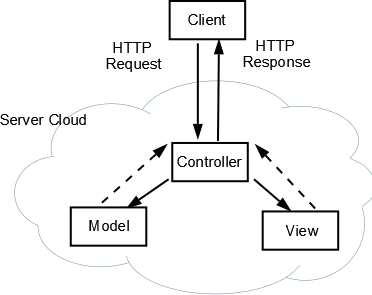
\includegraphics[width=8cm]{./Figures/mvc}
%  \rule{\textwidth}{0.005in}
  \caption{Model-View-Controller architectural pattern }
  \label{fig:mvc}
\end{figure}

The depicted pattern is a variant of the original Model-View-Controller pattern
\citep{RefWorks:28}. Instead of the model pushing updates to the view, the
controller pulls the data from the model, and passes model data to the
view. Therefore there are no connection between the model and the view, like in
the original MVC pattern.

In the following sections, the GAE and Django is described in terms of the MVC
pattern.

\subsection{Model}\label{sec:gae_model}
The models of the application declare the format of, and manipulate the data of
the application. The models are usually stored in a relational database. The
``database'' in GAE is special; it is not a normal relational database,
but a database based on Google's BigTable technology \citep{RefWorks:26}, called
datastore. The best way to think of the datastore is as a database of objects.

GAE comes with an API for datastore interaction, called Datastore API. The API
provides functionality to declare datastore entities, and declare their
properties, directly in Python, based on the \textit{\gls{gls:activerecord}}
pattern. Creating a data model with the Datastore API is easy. The datastore data
models are created reflectively, on their first import, by the GAE from Python
classes that inherits from the \verb|db.Model| class. This means a data model is
a Python class. The content of the data model is declared by defining class
attributes of the type \verb|Property| in the model class. An example model that
represents a surf spot is given in Listing~\ref{lst:spotModel}.

\lstset{language=Python}
\begin{lstlisting}[caption=Spot model,label=lst:spotModel]
from google.appengine.ext import db

class Spot(db.Model):
    name = db.StringProperty(required=True)
    point = db.GeoPtProperty(required=True)
\end{lstlisting}

The spot model uses the built-in property-classes to declare the properties of
the spot data model. The point property uses a richer semantic type
\verb|GeoPtProperty| used to store geographical points consisting of a latitude
and longitude. The API includes many such richer types, such as \verb|UserProperty|
and \verb|EmailProperty|.

References between tables in the datastore is defined by a reference property
variable in the referring class. The referenced entity is accessed as if it were
just an object reference. The GAE automatically creates indexes for the
references in order to increase the performance of reference look-ups.

\subsubsection{Queries}
\label{sec:queries}
Queries can be defined in two ways: 1) it is possible to define queries in a
SQL-like language called GQL, and 2) with a query object where the query is built
with methods. An example of the latter is the \verb|all| method in
Listing~\ref{lst:spotService}. GQL and query object are equally expressive,
however, comparing GQL with SQL is easier with GQL. The GQL syntax is given in
Listing~\ref{lst:gql}.  \lstset{language=SQL}
\begin{lstlisting}[caption=GQL grammar,label=lst:gql]
<gql> ::= SELECT [* | __key__] FROM <kind>
  [WHERE <condition> [AND <condition> ...]]
  [ORDER BY <property> [ASC | DESC] 
    [, <property> [ASC | DESC] ...]]
  [LIMIT [<offset>,]<count>]
  [OFFSET <offset>]

<condition> ::= <property> {< | <= | > | >= | = | != } <value>
<condition> ::= <property> IN <list>
<condition> ::= ANCESTOR IS <entity or key>
\end{lstlisting}
GQL is only concerned with fetching data. A GQL query always restricts by kind
 and zero or more property filters are applied. GQL is limited in comparison to
 SQL; notice the lack of JOINs, ORs, projections, and aggregation functions in
 the grammar. An important restriction is that when inequality filters are
 applied, they can only be on the same single property, e.g., a query with
 inequality filters on both a latitude and longitude is invalid.

GQL is subject to the design choice of scalability; to achieve scalability
Google removed the aforementioned functionality. The result is queries which %
%%
\begin{enumerate}
  \item avoid sorting records in memory \citep{Google:iodatastore}; 
  \item avoid expensive JOINs; and
  \item benefits from distributed servers; 
\end{enumerate}
%
This lack of expressive power is not a significant problem, however, it demands a
paradigm shift, because a relational SQL approach cannot be used; e.g., the
aggregate count function, unavailable in GQL, can be implemented by maintaining
an integer in the datastore of the count. Of course this could also be
implemented by fetching all objects into a list and doing a count of the objects
in the list, but this is exactly what is not meant to be done, because it demands
a lot of processing; in addition, the data set of queries is restricted to 1000
entities, making the result invalid when that upper bound is hit.

\subsection{View}
\label{sec:view}
The view layer in Django consist of Django templates. A Django template consists
of
\begin{itemize}
  \item regular text (HTML, JavaScript, etc.);
  \item programming constructs for sticking in values in the template, always
  resident inside \verb|{{ }}|; and
  \item control flow constructs called block tags \citep{django:templates},
always resident inside \verb||.
\end{itemize}
When a template is rendered a dictionary is passed to it, the values are stuck
into the template, properties are resolved, and a text document is returned.  

A template that will render all spots (given to it in a dictionary) in JSON
 format is given in Listing~\ref{lst:spotsJs}. The template takes advantage of
 the \verb|for| block tag to iterate through all the spots in a given
 dictionary. For every spot the template outputs attribute name value pairs. The
 \verb|if| block tag uses \verb|forloop.last| to check whether the current
 iteration element is not the last, and outputs a comma if so; without the check
 it would return invalid JSON.

%% The template language supports component driven design, by enabling
%% inheritance between templates and inclusion of other templates in a
%% template.

\lstset{language={}, showspaces=false, showtabs=false}
\begin{lstlisting}[caption=Django template,label=lst:spotsJs]
[ 
  
    {
      "id": "{{ spot.key.id }}",
      "name": "{{ spot.name }}",
      "lat": {{ spot.point.lat }},
      "lng": {{ spot.point.lon }}
    }
    ,
  
]
\end{lstlisting}

\subsection{Controller}\label{sec:controller}
Controllers mediate between views and models. A controller consists in a
dispatcher and a request handler. After the dispatcher has passed a request to
the relevant handler, the handler 
\begin{enumerate}
  \item gets relevant data from the models;
  \item parses the data to the view; and
  \item returns the rendered view in a response.
\end{enumerate}

GAE and Django handles much of the controller logic, GAE maps \gls{gls:uri}s to
an application, and Django maps \gls{gls:uri}s to request handlers by regular
expressions. The request handlers, together with the regular expression mappings
from URI to request handler, is the part of the controller that the developer is
responsible for. An example of a request handler is given in
Listing~\ref{lst:spotService}. The request handler gets all the spots from the
datastore, by using the query object interface of the Spot model class. The data
is parsed on as a dictionary to the template which is rendered, and the result
returned to the client in a response object.

\lstset{language=Python}
\begin{lstlisting}[caption=Spot service handler,label=lst:spotService]
"""Returns spots in JSON format"""
def index(request):
    data = {'spots': models.Spot.all()}
    response = shortcuts.render_to_response('spots/spots.js', data)
    return response
\end{lstlisting}

\section{Putting it together}
Given the model snippets, the controller snippets and the view snippets in the
last sections, we almost have a complete GAE Web application\footnote{We assume
that \verb|app-engine-patch| is downloaded and setup}. What remain are to%
%
\begin{enumerate}
  \item register the application with an \gls{gls:uri}; and
  \item register the event handler with an \gls{gls:uri}.
\end{enumerate}
%
In Listing~\ref{lst:main} the URI to request handler file is shown.

\begin{lstlisting}[caption=URI to request handler,label=lst:main]
urlpatterns = patterns('',
    (r'^spots/$', index),
)
\end{lstlisting}

Each application in the GAE has an application descriptor named
\verb|app.yaml|. An example of such a file is given in
Listing~\ref{lst:app.yaml}. The file registers the main module with every
\gls{gls:uri} request to the application. As shown in Figure~\ref{fig:webapp},
several applications can exist; \verb|app.yaml| is the place where we route to
the appropriate, specified under \verb|handlers|. In addition, the application
name and version are stated here, which are used when uploading the application to
the server.

\begin{lstlisting}[caption=app.yaml configuration file,label=lst:app.yaml]
application: welovewind
version: 1
runtime: python
api_version: 1

handlers:
- url: /.*
  script: common/appenginepatch/main.py
\end{lstlisting}

After registering the application at \url{http://appengine.google.com}, the
application is put into production by running a single command; type
\begin{verbatim}
manage.py update
\end{verbatim}
in the directory of the application, and the application is online, see
Figure~\ref{fig:spots_service}.

\begin{figure}[htbp]
	\centering
	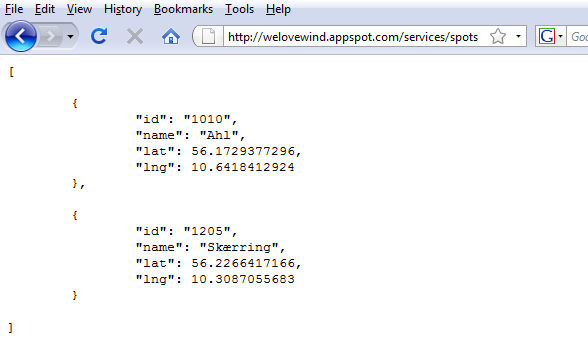
\includegraphics[width=11cm]{./Figures/spots_service}
%        \rule{\textwidth}{0.005in}
	\caption{Spots Service}
	\label{fig:spots_service}
\end{figure}

\section{Further GAE prerequisites}
This section presents GAE prerequisites for later sections. The reader can skip
the section for now and revisit it when the prerequisites are used in later
sections.

\subsection{Unique Properties}\label{sec:unique_props}
In the datastore there is no built-in option that enforces unique properties on
the models. Per design there is only one unique property namely the key of the
model. This leaves two possibilities for implementing unique constraints:

\begin{enumerate}
  \item simulate unique properties in Python\footnote{An example of a Python
  programmatic implementation of unique properties is available at:
  \url{http://appengine-cookbook.appspot.com/recipe/get-or-insert-entity-by-unique-properties/}};
  or
  \item incorporate the unique property in the key name.
\end{enumerate}

Simulating unique properties results in a fairly clean solution, however, it has
the huge flaw that there is no possible way of ensuring that the properties are
indeed unique since they are simulated. This is a problem if the solution is
applied in a concurrent environment and uniqueness guarantees are essential. The
second solution is obviously a solution to a recurring problem and we describe
this in the following.

As mentioned, the datastore ensures exactly one unique property per instance: the
key name of the instance. The Datastore API provides a transactional method on
models which either gets or inserts an instance based on the key name. We use the
method to ensure uniqueness by incorporating the unique constraints in the
keyname.

Listing~\ref{lst:unique_props_keyname} shows the implementation of unique
properties for the \verb|Forecast| weather data class. It is based on the concept
that a forecast point only should have one forecast for each time delta (the
difference between calculation time and forecast time). The delta is incorporated
into the key name to ensure the uniqueness.

The class method \verb|key_name| returns the unique key name to use for the
entity; the key name is the URI of the forecast resource. The method is used in
\verb|update_or_insert|, which as the first step calls it to get the key name
from the given arguments. The key name is used as input to \verb|get_or_insert|
that gets or creates a forecast with the specified time delta and forecast point,
now incorporated in the key name.

Instead of only getting an entity when the entity exist the authors
implementation updates the entity both when entities are updated and created. To
find out whether the entity exists a \verb|is_new| key word is passed to the
entity model. Since the key word is used only when the entity is unsaved the
property is only set to \verb|True| in this case.


\begin{lstlisting}[label=lst:unique_props_keyname,caption=Forecast with unique properties]
class Forecast(AbstractWeatherData):
  
  def __init__(self, is_new = False, **kwds):
    self.is_new = is_new
    super(Model, self).__init__(**kwds)

  (...)

  @classmethod
  def key_name(cls, calculation_time, forecast_time, forecast_point):
    time_delta = wlwtime.timeDifferenceInHours(calculation_time, forecast_time)
    owner = forecast_point.key().name()
    return '%s/forecasts/time_delta/%s' % (owner, time_delta)

  @classmethod
  def update_or_insert(cls, calculation_time, **kwds):
    '''Update or insert forecast weather data.
          
    Args:
      calculation_time: forecast calc. time (datetime).
      **kwds: Key word arguments to pass to the instance and 
        update / init the value of.
          
    Returns:
      Updated / new instance.
    '''
    key_name = Forecast.key_name(calculation_time, 
             kwds['time'], kwds['forecast_point'])
    entity = super(Forecast, cls).get_or_insert(key_name, is_new=True, **kwds)
    if not entity.is_new:
      for prop in kwds.keys():
        setattr(entity, prop, kwds[prop])
      entity.put()
    return entity
\end{lstlisting} 

\subsection{Pagination}\label{gae:pagination}
Pagination is the process of splitting up content into several resources. The GAE
limits the number of returned results of a query and restricts the duration of a
request. Because of the restrictions pagination is a must have.

Django comes with a built-in paginator class that handles pagination. The
paginator takes a complete list of objects and provides methods to get specific
pages. However, since the class takes a list of all the objects that should be
paginated it causes a slowdown as more and more objects are in the list; in
addition, since the datastore is limited to a result set of 1000, the paginator
is not able to access list objects beyond the limit.

The author's initial (un-scalable) solution was a slightly changed version of the
paginator that only retrieved objects that belonged to the current page plus one
more object. The extra object is used to evaluate whether the current page has a
next page. The new paginator instead of taking a list of objects, takes a query
as argument. The paginator then puts the relevant filters on the query object to
retrieve only the objects needed for the page requested plus the additional
entity to evaluate whether the page has an additional page. The modified
paginator fetches objects with the following query:
\begin{verbatim}
objects =  query.fetch(limit=per_page + 1,
                       offset=(self.page_number-1) * per_page)
\end{verbatim}
This query is un-scalable. Specifying an offset merely chops off entities in the
result set, however, the entities are still fetched from the datastore. That the
offset argument is provided is just confusing.

The only way to do scalable pagination is paging based on an indexed property and
limiting the number of entities. Following pages continues from the last value
(in the previous page) in terms of the ordering using an in-equality filter on
that property. We put it to use in Section~\ref{sec:models}.


\subsection{Timezones}\label{sec:gae_tz}
All times in the datastore are stored in Coordinated Universal Time (UTC). When
displaying times to the user the application should convert the UTC times to the
local times. The easiest way to convert between UTC and the timezone of the user
is by using JavaScript. However, JavaScript is not always available and then a
conversion on the server is needed.

Converting between timezones on the server is complicated since Python does not
come with logic to handle the different timezones. It merely provides an abstract
interface. What is needed is a complete database of the politically decided
timezone offsets and daylight saving times. The tz database, or Olson Timezone
database, is a continuously maintained database of timezone info. In Python the
\verb|pytz|\footnote{\url{http://pypi.python.org/pypi/pytz/}} module wraps the tz
database and provides access to the Olson database. The \verb|pytz| module is not
included in the Python Standard Library.

\verb|pytz| includes over 500 hundred files. The GAE has a restriction of 1000
uploaded files; the limit is quickly crossed when including pytz. All files
except four are binary timezone definitions belonging to the \verb|tz|
database. A blog entry\footnote{\url{http://takashi-matsuo.blogspot.com/2008/07/using-newest-zipped-pytz-on-gae.html}}
describes how to circumvent the problem by zipping all the timezone files, and
include logic to unzip them during runtime.

The GAE provides a distributed memory cache -- memcache -- which is a distributed
hash table. Unzipped timezones are obvious subjects for caching in the
distributed memory. Saving timezones in the memcache avoids the overhead in
unzipping data from the \verb|tz| database repeatedly.

Listing~\ref{lst:pytz} shows the single method in \verb|pytz| we overwrite to
incorporate the two changes: the changed method reads timezone definitions from
the zipped archive of timezones \verb|zoneinfo.zip|, and caches the result in the
memcache. The code is based on an example from the Google App Engine Cookbook
\footnote{\url{http://appengine-cookbook.appspot.com/recipe/caching-pytz-helper/}}.

\begin{lstlisting}[caption=Altered pytz,label=lst:pytz]
def open_resource(name):
    """Open a resource from the zoneinfo subdir for reading.

    """
    import zipfile
    from cStringIO import StringIO
    name_parts = name.lstrip('/').split('/')
    for part in name_parts:
        if part == os.path.pardir or os.path.sep in part:
            raise ValueError('Bad path segment: %r' % part)
    cache_key = "tzinfo/%s/%s" % (OLSON_VERSION, name)
    zoneinfo_contents = memcache.get(cache_key)
    if zoneinfo_contents is None:
        zoneinfo = zipfile.ZipFile(os.path.join(os.path.dirname(__file__), 
            'zoneinfo.zip'))
        zoneinfo_contents = zoneinfo.read(os.path.join(
            'zoneinfo', *name_parts).replace('\\','/'))
        memcache.add(cache_key, zoneinfo_contents)
    return StringIO(zoneinfo_contents)
(...)

# We don't need this, since we are including all tzinfo files
#all_timezones = [
#        tz for tz in all_timezones if resource_exists(tz)]

\end{lstlisting}

\verb|pytz| iterates through all timezone files when it is initialized, checking
whether every timezone file exist, we remove this as we have included the whole
tz database; avoiding the latency of unzipping over 500 files everytime the
server is started. The removed code is also shown in Listing~\ref{lst:pytz}.

With \verb|pytz| in place we are armed to convert between
timezones. Listing~\ref{lst:utc_to_local} shows how to convert from the times
stored in the datastore, UTC, to a local timezone. Datetimes stored in the datastore
does not have timezone information in them; before converting to local time it
must be added. After the datetime is enriched with timezone information it is
converted to local time with \verb|astimezone(tz)|: the function adjusts a
datetime according to the given timezone.

\begin{lstlisting}[caption=Converting datastore time to localtime,label=lst:utc_to_local]
>>> from pytz import timezone
>>> from datetime import datetime
>>> def local_time(utc_dt, tz_string):
...     utc = timezone('UTC')
...     utc_dt = utc_dt.replace(tzinfo=utc)
...     tz = timezone(tz_string)
...     return utc_dt.astimezone(tz)
...
>>> utc = datetime.utcnow()
>>> utc
datetime.datetime(2009, 5, 5, 6, 30, 53, 793000)
>>> lt = local_time(utc, 'Europe/Copenhagen')
>>> lt
datetime.datetime(2009, 5, 5, 8, 30, 53, 793000, tzinfo=<DstTzInfo 'Europe/Copenhagen' CEST+2:00:00 DST>)
\end{lstlisting}

\verb|pytz| is put into action in Section~\ref{sec:models}, where we also
describe how to get the relevant timezone string, e.g.,
\verb|'Europe/Copenhagen'|.

%% \section{Cron jobs}
%% Long running requests on GAE is aborted, and a message is sent to the
%% user. This poses a problem for the welovewind webapp, as the app has to
%% fetch data at several external resources. Obviously, this can't be done
%% be fetching external data from the source every time it's
%% needed. Instead we keep track of when to fetch new data and insert this
%% into the datastore.

%% "spawn a sub-process or thread. A web request to an application must be handled in a
%% single process within a few seconds. Processes that take a very long time to respond
%% are terminated to avoid overloading the web server."


%% Then sign up for one of those web-site 
%% monitoring services that ping your website to see that it's alive

%% \url{http://schedulerservice.appspot.com/about}

%%\section{Testing}

%%\section{Comet, AJAX Push}

%%\section{Comparison to similar offerings}

\section{Summary}
In this chapter we have presented the GAE and the Web application framework,
Django. GAE and Django is used in the rest of the dissertation as the basis upon
which we shall build several elements that will support the aspiration of assisting
wind- and kitesurfers. The chapter also presented GAE solutions to the common
problems of pagination, unique properties of data models, and conversion of times
to another timezone.
